%
% Chapter 10
%

\chapter{SYSTEMATIC UNCERTAINTIES}
Systematic uncertainties, often referred to as ``systematics'', are the uncertainties which are introduced as a result of inaccurate and imprecise measurements
inherent to the system. Systematics are distinct from the uncertainties driven by randomness, which are referred to as statistical uncertainties.
The systematics in this analysis can be classified as being purely theoretical, purely experimental, or a mixture of both, and include
the uncertainties on the theoretical understanding of rates and discriminant shapes for the MC-based signal and background predictions,
the uncertainties from control regions and extrapolations used in the data-driven background predictions
and finally the uncertainties resulting from data-to-MC agreement in scale factors, and jet energy corrections, respectively.

Systematic uncertainties are accounted for in the maximum likelihood fit through nuisance parameters, where each nuisance parameter represents a systematic uncertainty.
Uncertainties on the overall normalization of the discriminant are called rate systematics, while uncertainties on
the shape of the discriminant are called shape systematics\footnote{Some shape systematics also vary the overall normalization.}.
The rate uncertainty scales all bins of the discriminant by the same factor, while the shape uncertainty varies individual bins separately,
thus changing the shape of the discriminant.

The correlations, or lack thereof, of each of the 274 systematic uncertainties in this analysis are accounted for in the likelihood fit with the nuisance parameters. 
Rate uncertainties arising from the same source, are treated as fully correlated across event categories, and are represented by the same nuisance parameter.
Shape uncertainties are treated as fully correlated between bins of the discrmininant within each category and are represented by nuisance parameters corresponding to
each category. The bin-by-bin shape uncertainties, which account for large statistical uncertainty from limited event yields in a bin of the discriminant, are treated as uncorrelated
and each uncertainty is represented by a unique nuisance parameter.  


\section{Theoretical Uncertainties}
The theoretical uncertainties in this analysis arise from the NLO calculation of the cross section for the signal and MC-based background predictions.
For \tth signal, these uncertainties amount to +5.8$\%$ -9.2$\%$ from unknown higher order terms in the perturbative expansion and an additional 3.6$\%$ uncertainty for the
PDFs and the scale ($\alpha_{s}$). For the leading MC background of \ttw and \ttz, the cross section uncertainties are 12$\%$ and 10$\%$ respectively, with
scale uncertainties of 2$\%$ and 3$\%$ respectively~\cite{xsec_uncert}.

The multiboson processes that form a significant fraction of the remaining MC backgrounds are predicted at NLO accuracy and have theoretical uncertainties
similar to the signal and leading background samples. Many of these processes, such as $WZ$ and $ZZ$ do not contain b-jets at leading order, and the flavor
composition of their additional jets in part affects their yields in this signal region, which requires at least one b-tagged jet. 
The fraction of predicted WZ events in the signal region that contain b-jets is 18$\%$, 37$\%$ in the b-loose and b-tight categories respectively, with the
remaining fraction events due to mis-tagged gluon, light flavor, and charm jets. 
The leading theoretical uncertainties for multiboson backgrounds therefore arise from the modeling of the heavy flavor content of the jets,
in addition to the scale and PDF uncertainties (approximately $20\%$). Additionally we factor in the experimental uncertainty on the b-tagging efficiency
which ranges from $10\%-40\%$. We conservatively combine both of these into a single uncertainty of 100$\%$ on the $WZ$ background. The largest remaining SM
backgrounds contain two b-jets, while the others contain one or fewer b-jets and have very small contributions to signal region. We therefore
assign a 50$\%$ uncertainty to all other background MC predictions. 

\section{Scale Factor Uncertainties}
Scale factor systematics represent the uncertainty associated with the agreement between data and MC. In this analysis,
scale factor uncertainties enter the fit in the form of both rate and shape systematics. Scale factor uncertainties are assesed for trigger efficiency,
lepton selection efficieny, b-tagging efficiency. The trigger efficiencies between data and MC show nearly perfect agreement, and the uncertainties on the corresponding
scale factors amount to 2$\%$ - which is propagated as a rate uncertainty.

The uncertainties on the b-tagging scale factors are assessed for heavy flavor, charm flavor and light flavor separately.
These uncertainties include the jet energy scale (JES), where the scale factors are re-derived with JES shifted up and down,
the purity, where the light (heavy) flavor contamination for heavy (light) flavor scale factors is shifted up and down by 20$\%$,
and finally from linear and quadratic statistical fluctuations in both data and MC. 
These uncertainties are propagated to the fit as shape uncertainties and vary between 10$\%$-40$\%$.

The uncertainties on the jet energy corrections (JEC) are calculated by shifting the weight of each jet up and down
by $\pm$1$\sigma$ and re-calculating the signal region yields. The uncertainties from the JEC amount to approximately 4$\%$. 

\section{Data-driven Background Uncertainties}
The systematics associated with the data-driven background control regions are the largest uncertainties in this analysis. 
Several checks are performed to estimate the uncertainties related to the data/MC agreement in the control regions used for
the data-driven background estimations.
Additional systematics are introduced to account for uncertainties on lepton kinematic variables and their effects on the resulting fake rate. 

For the background due to non prompt leptons, rate uncertainties are assessed for the data/MC agreement of the measured fake rate
and are evaluated separately for electrons and muons in the b-tight and b-loose signal regions.
The fake rates measured in data are compared with those measured in MC in Figure~\ref{fig:fakerate}.
The uncertainties for the electron (muon) fake rates range from 10\% to 30\% (from 20\% to 40\%) depending on the analysis category, and are larger in the b-tight categories.
Shape uncertainties on the fake rate measurement are assessed separately for muons and electrons by varying the fake rates themselves,
and separately varying the lepton kinematic variables which affect the fake rate, specifically lepton \pt and $|\eta|$. All of these quantities are varied up and down
within their uncertainties ($\pm$1$\sigma$), and the discriminant shape is reproduced for each variation at fixed normalization with respect to the nominal shape.
These variations are shown in Figure~\ref{fig:FRvars_shape}.

\begin{figure}[htb]
        \centering 
        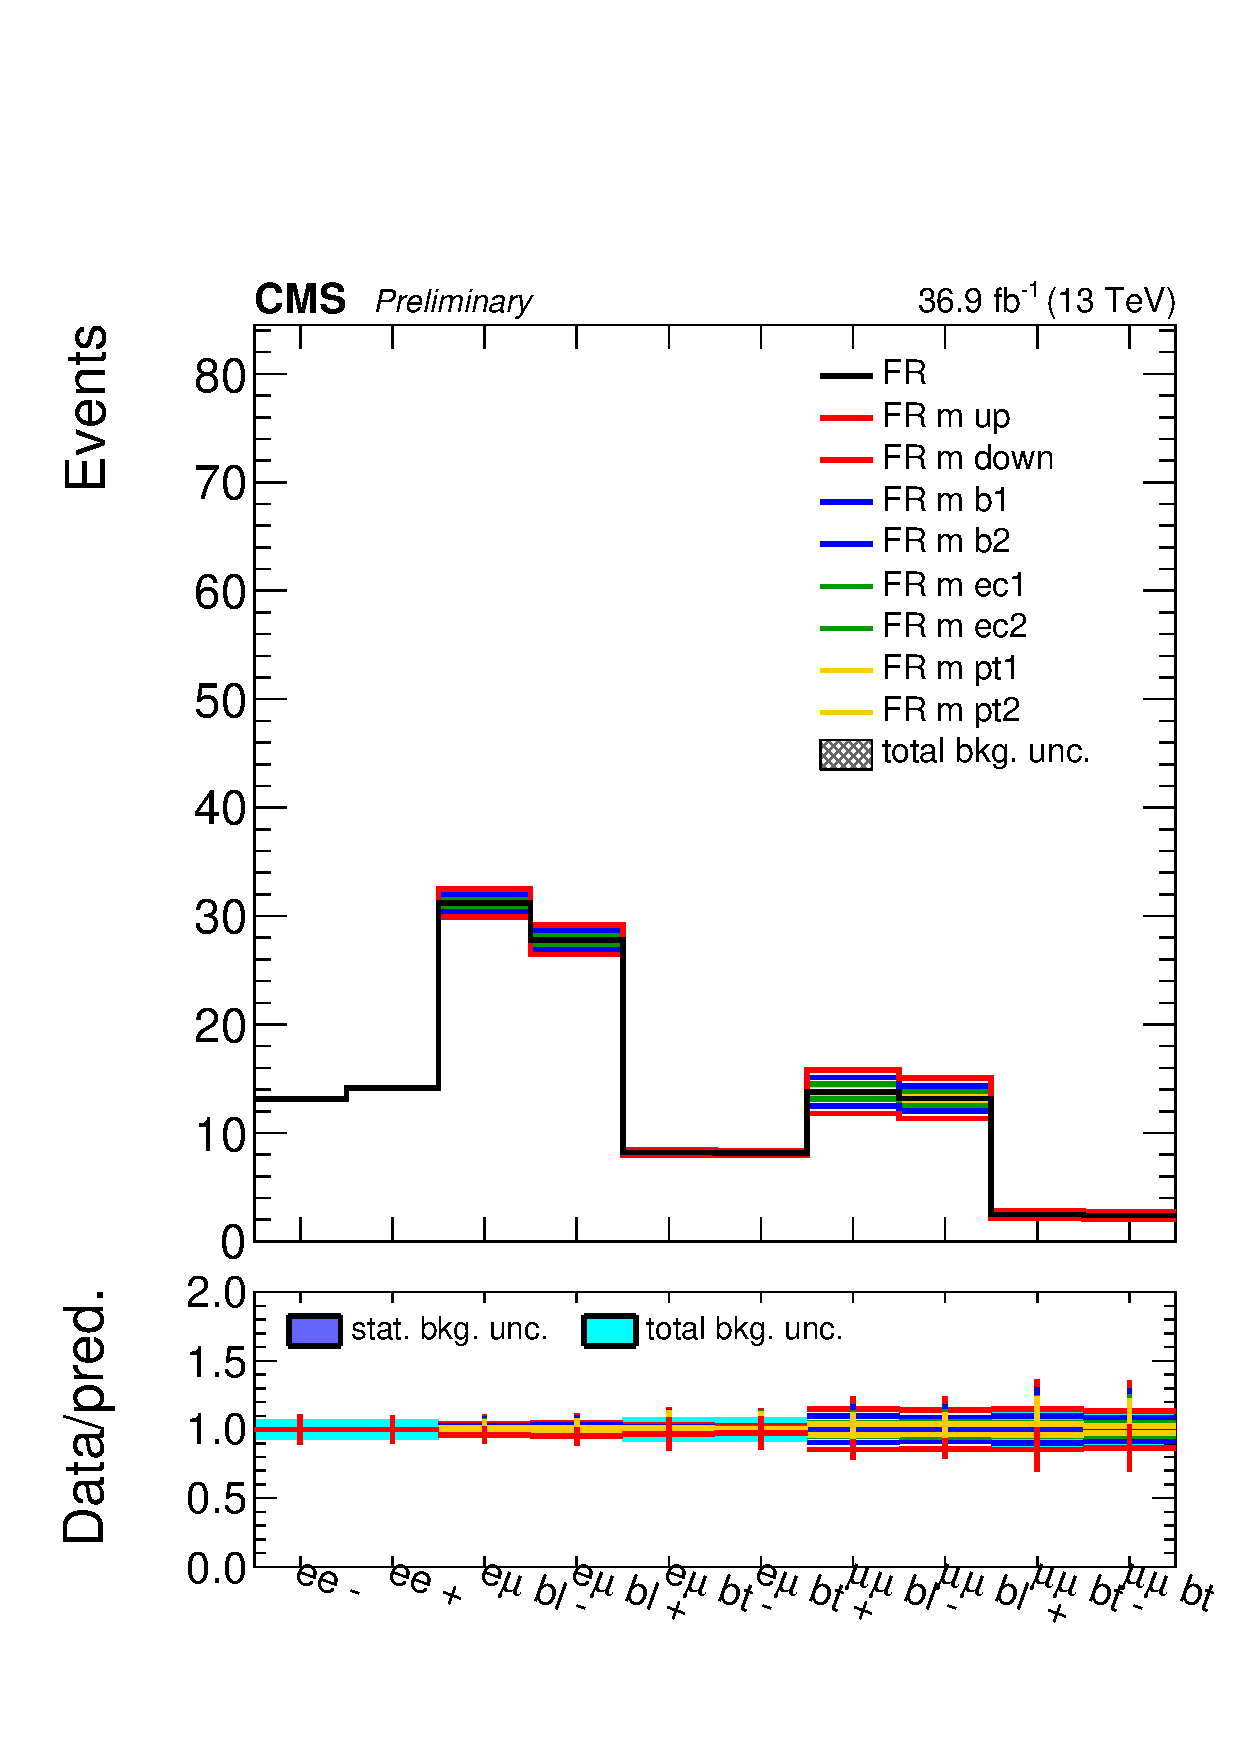
\includegraphics[width=0.32\textwidth]{ch10_figs/2lep_mu_catIndex.pdf}
        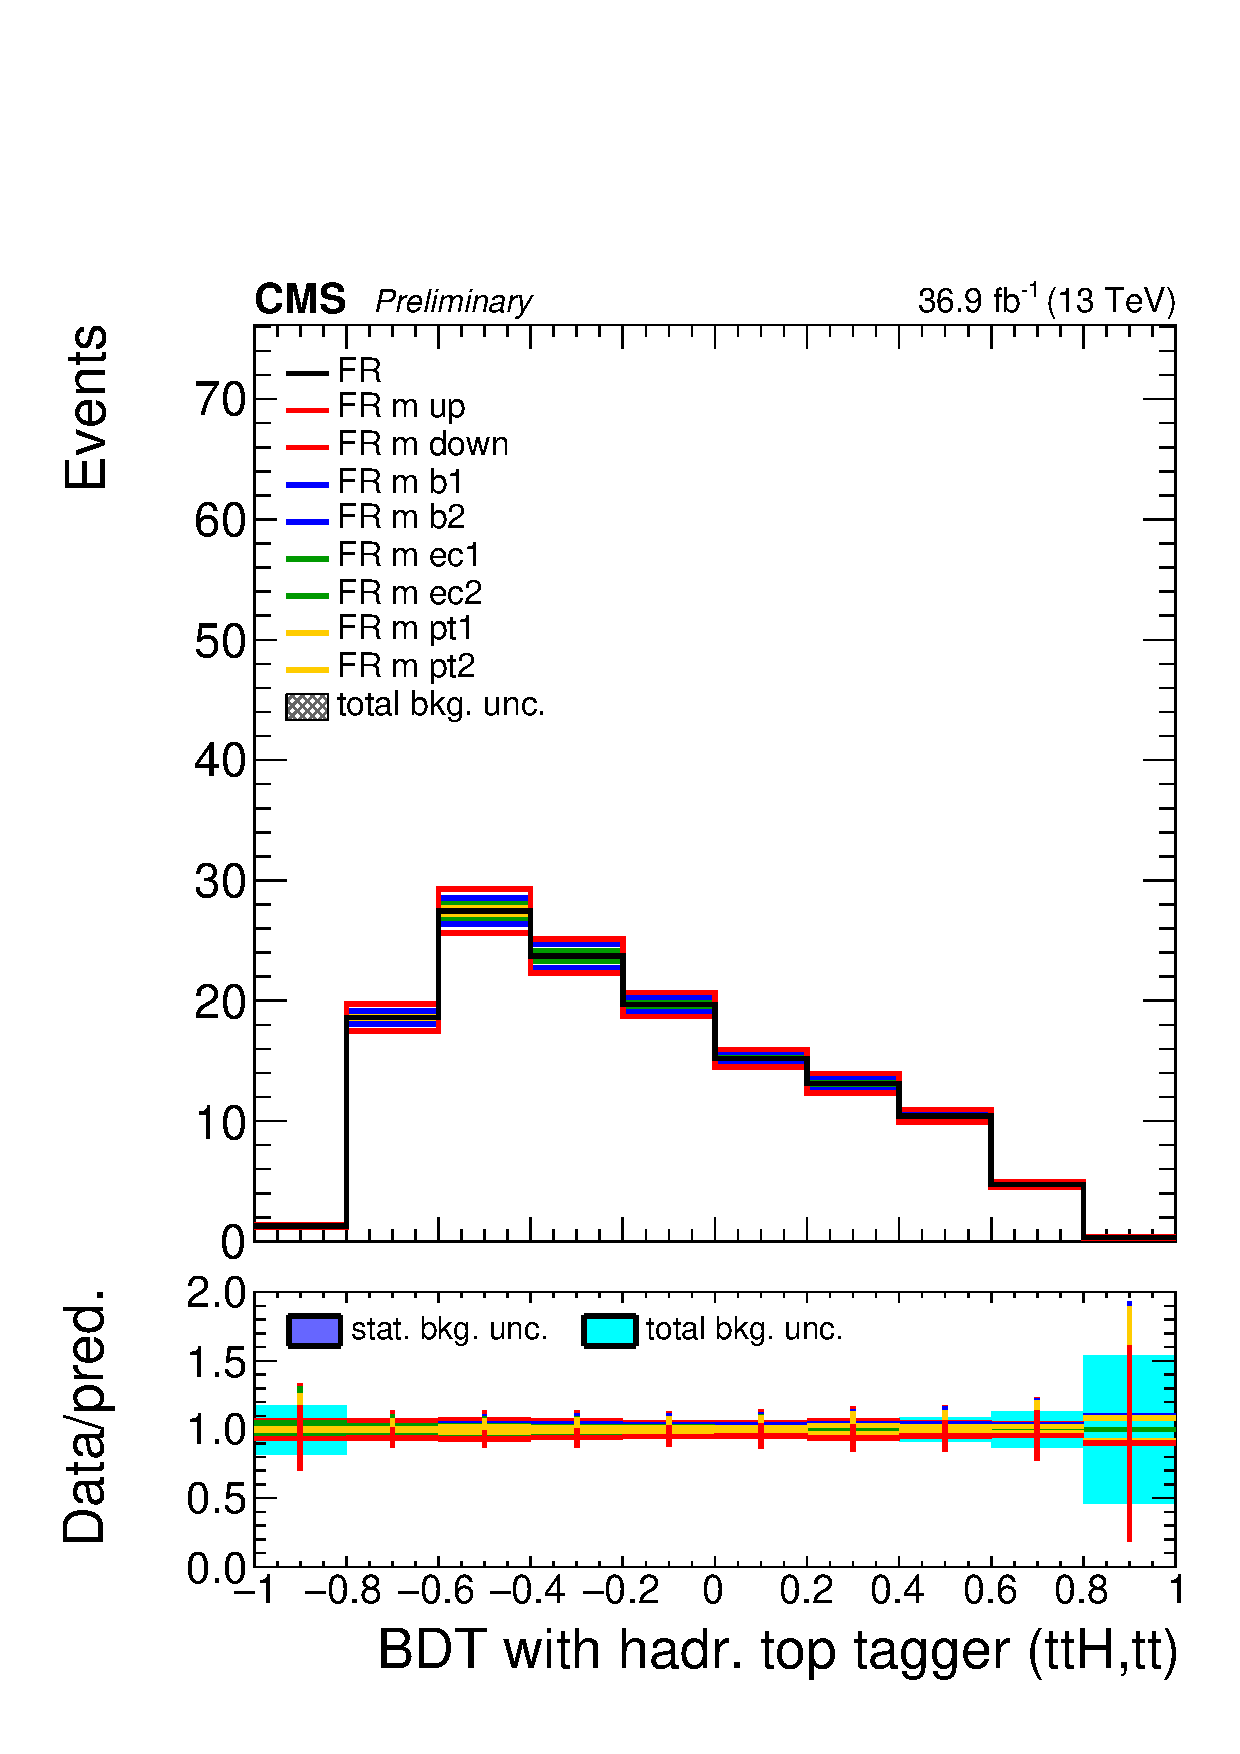
\includegraphics[width=0.32\textwidth]{ch10_figs/kinMVA_2lss_mu_ttbar_withBDTv8.pdf}
        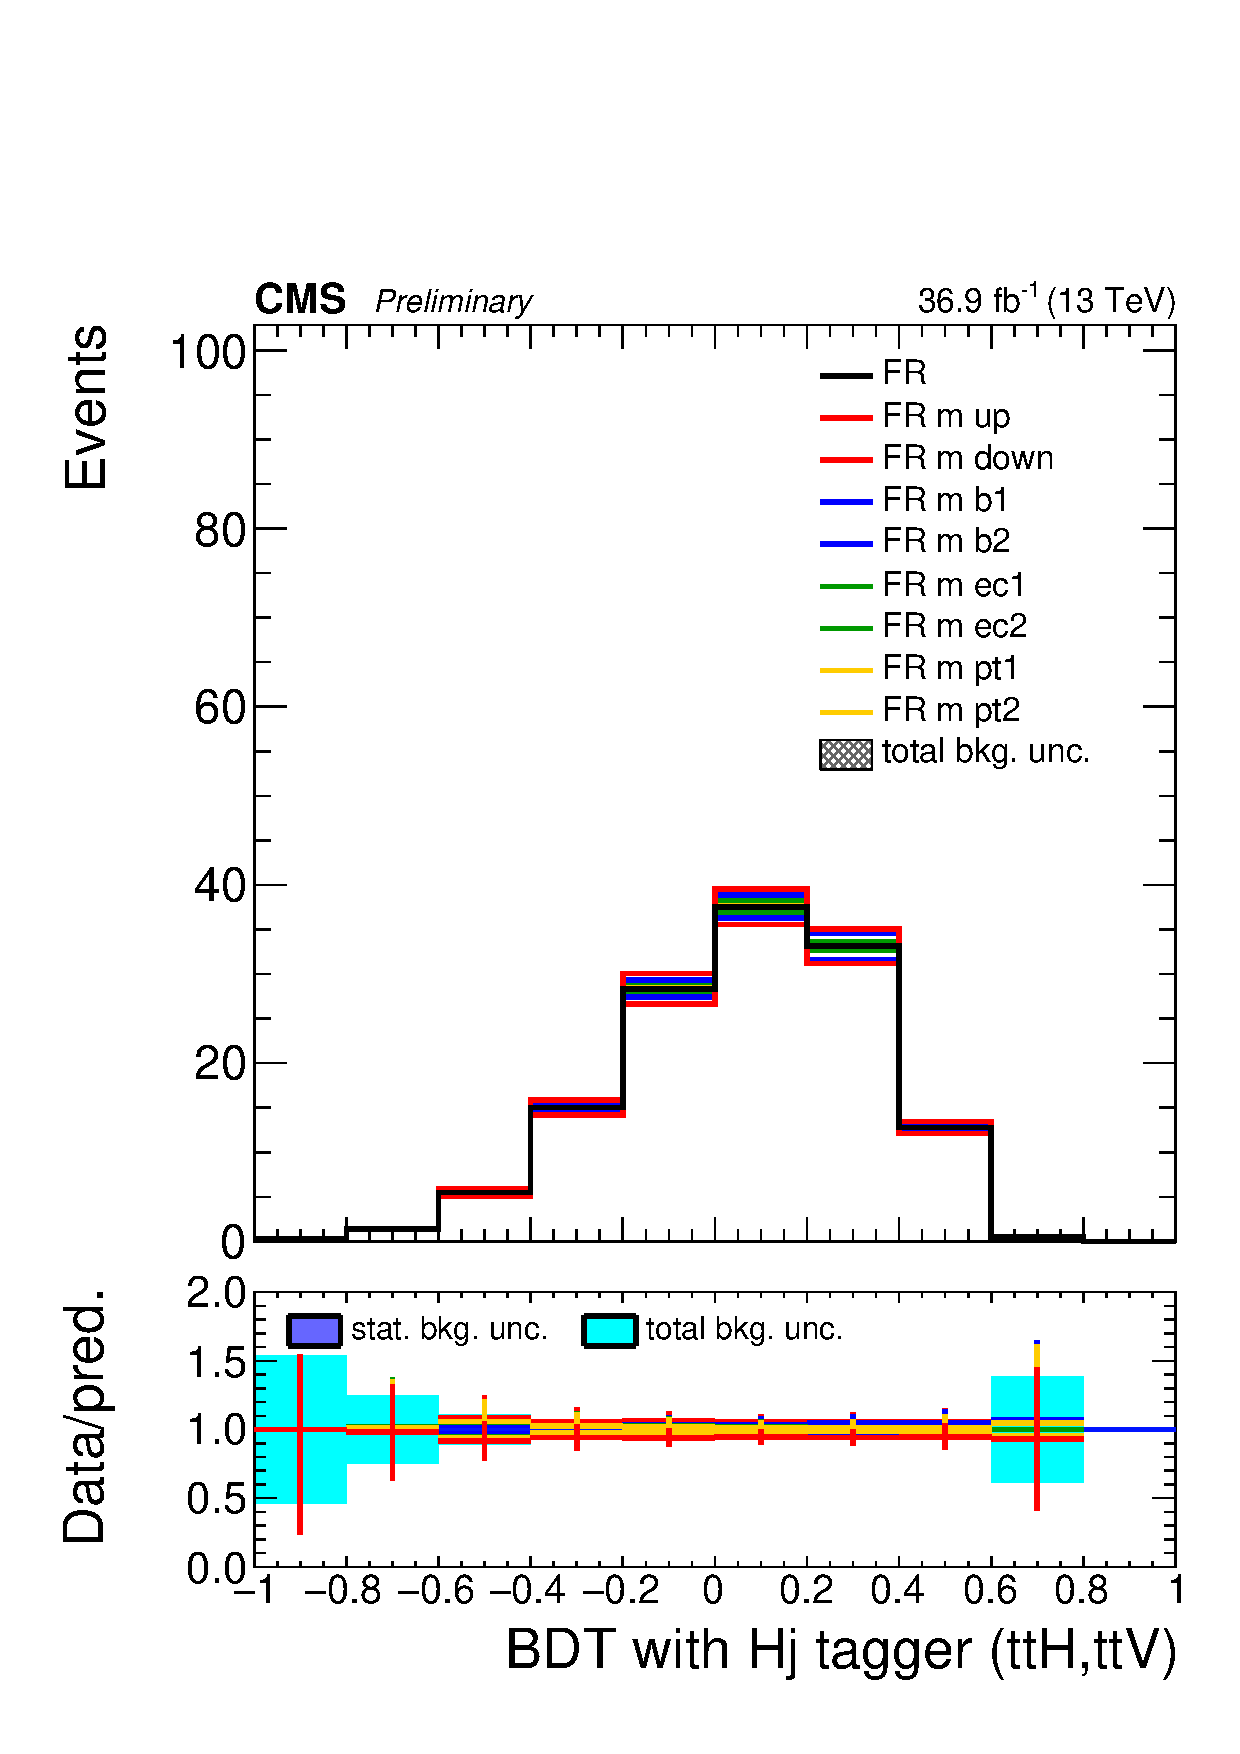
\includegraphics[width=0.32\textwidth]{ch10_figs/kinMVA_2lss_mu_ttV_withHj.pdf}\\
        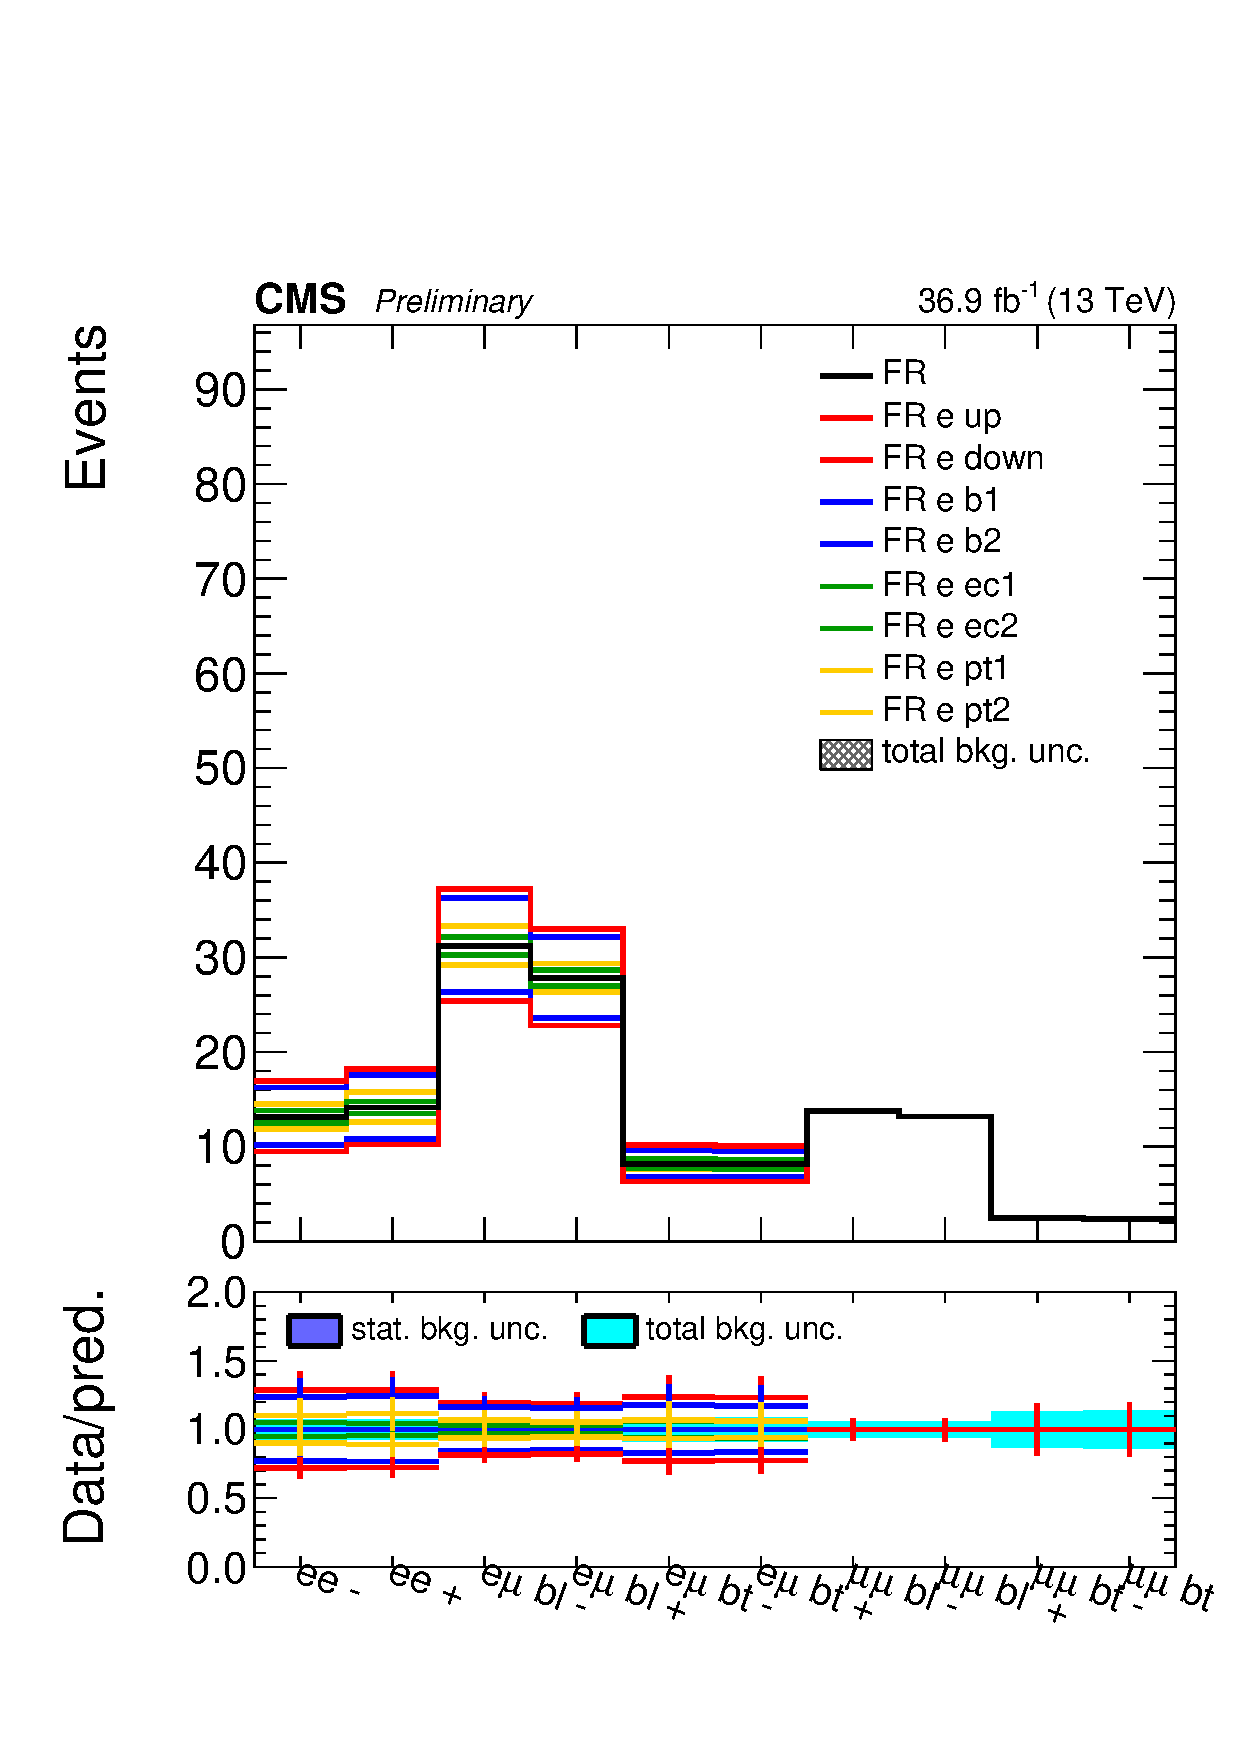
\includegraphics[width=0.32\textwidth]{ch10_figs/2lep_e_catIndex.pdf}
        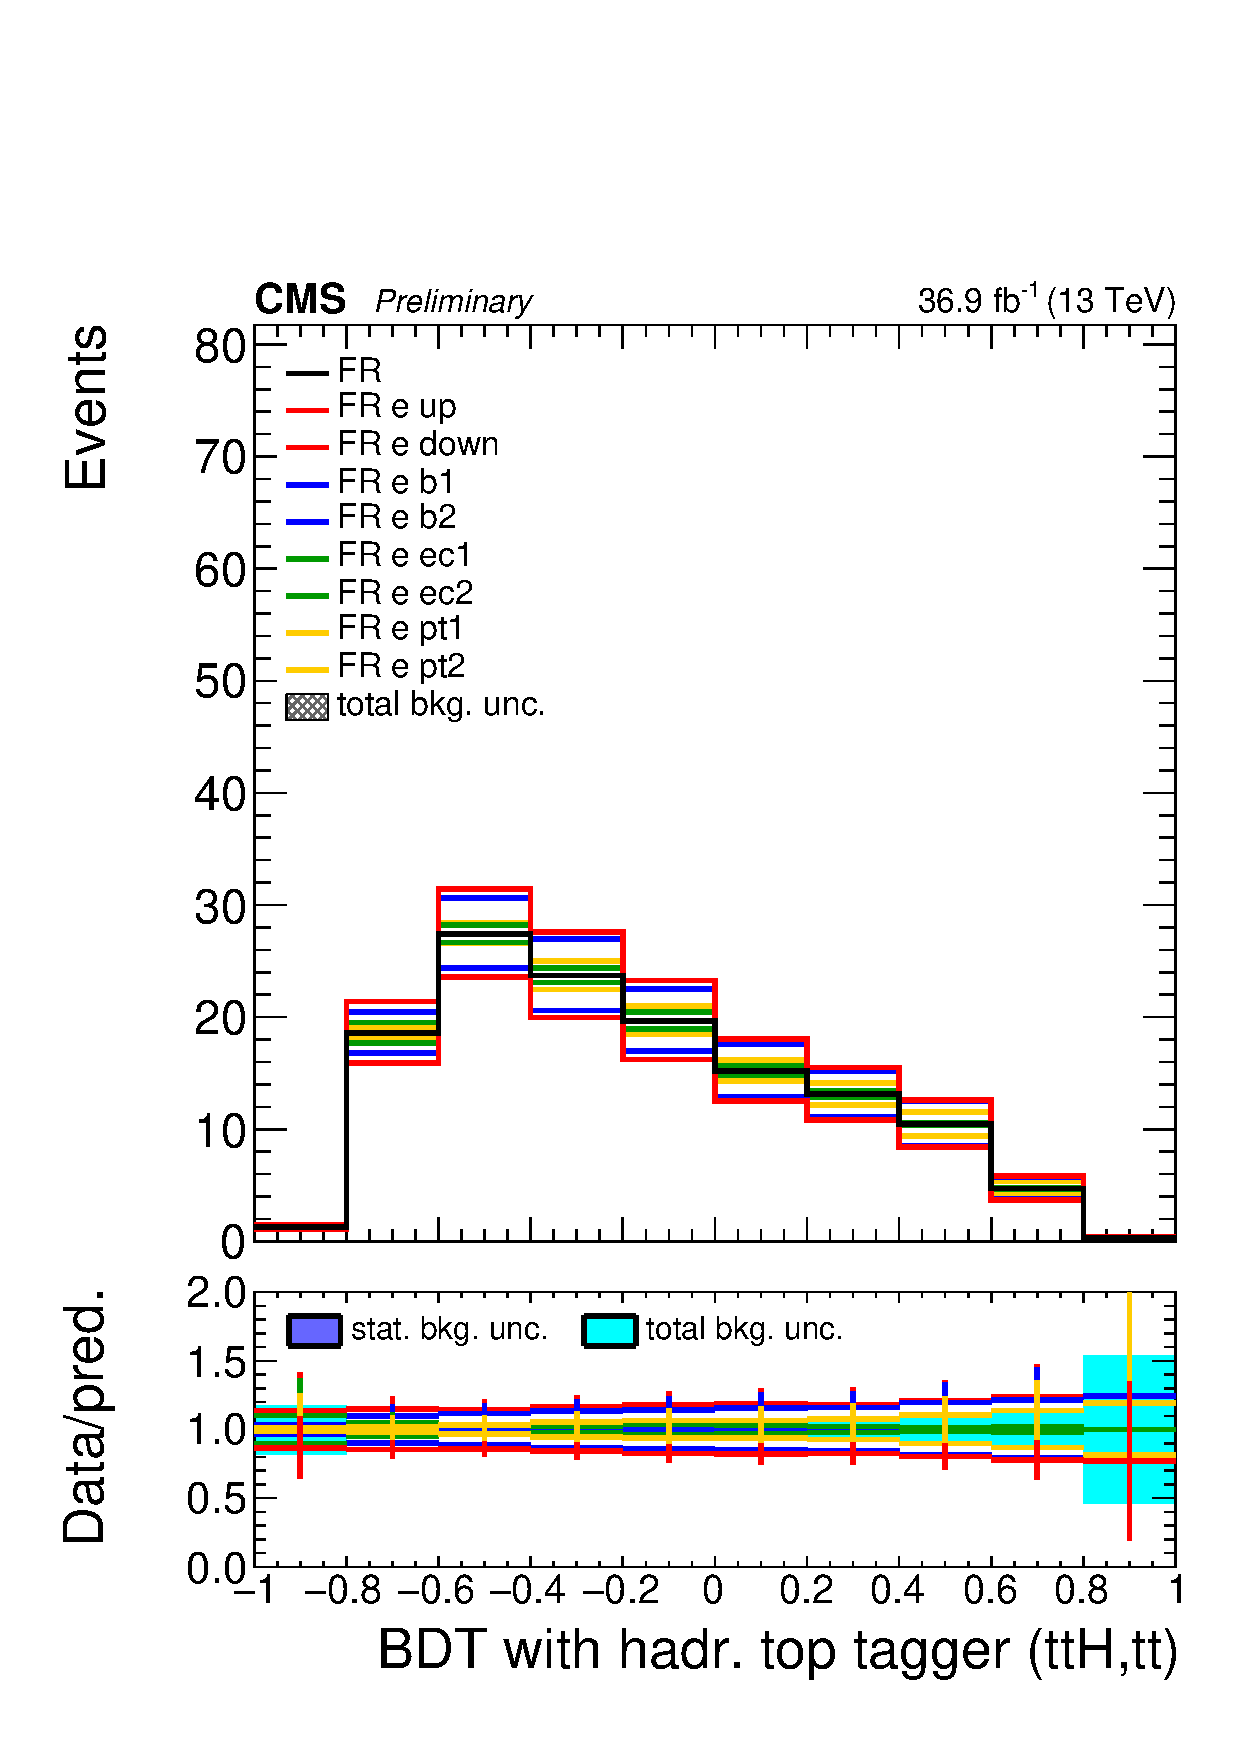
\includegraphics[width=0.32\textwidth]{ch10_figs/kinMVA_2lss_e_ttbar_withBDTv8.pdf}
        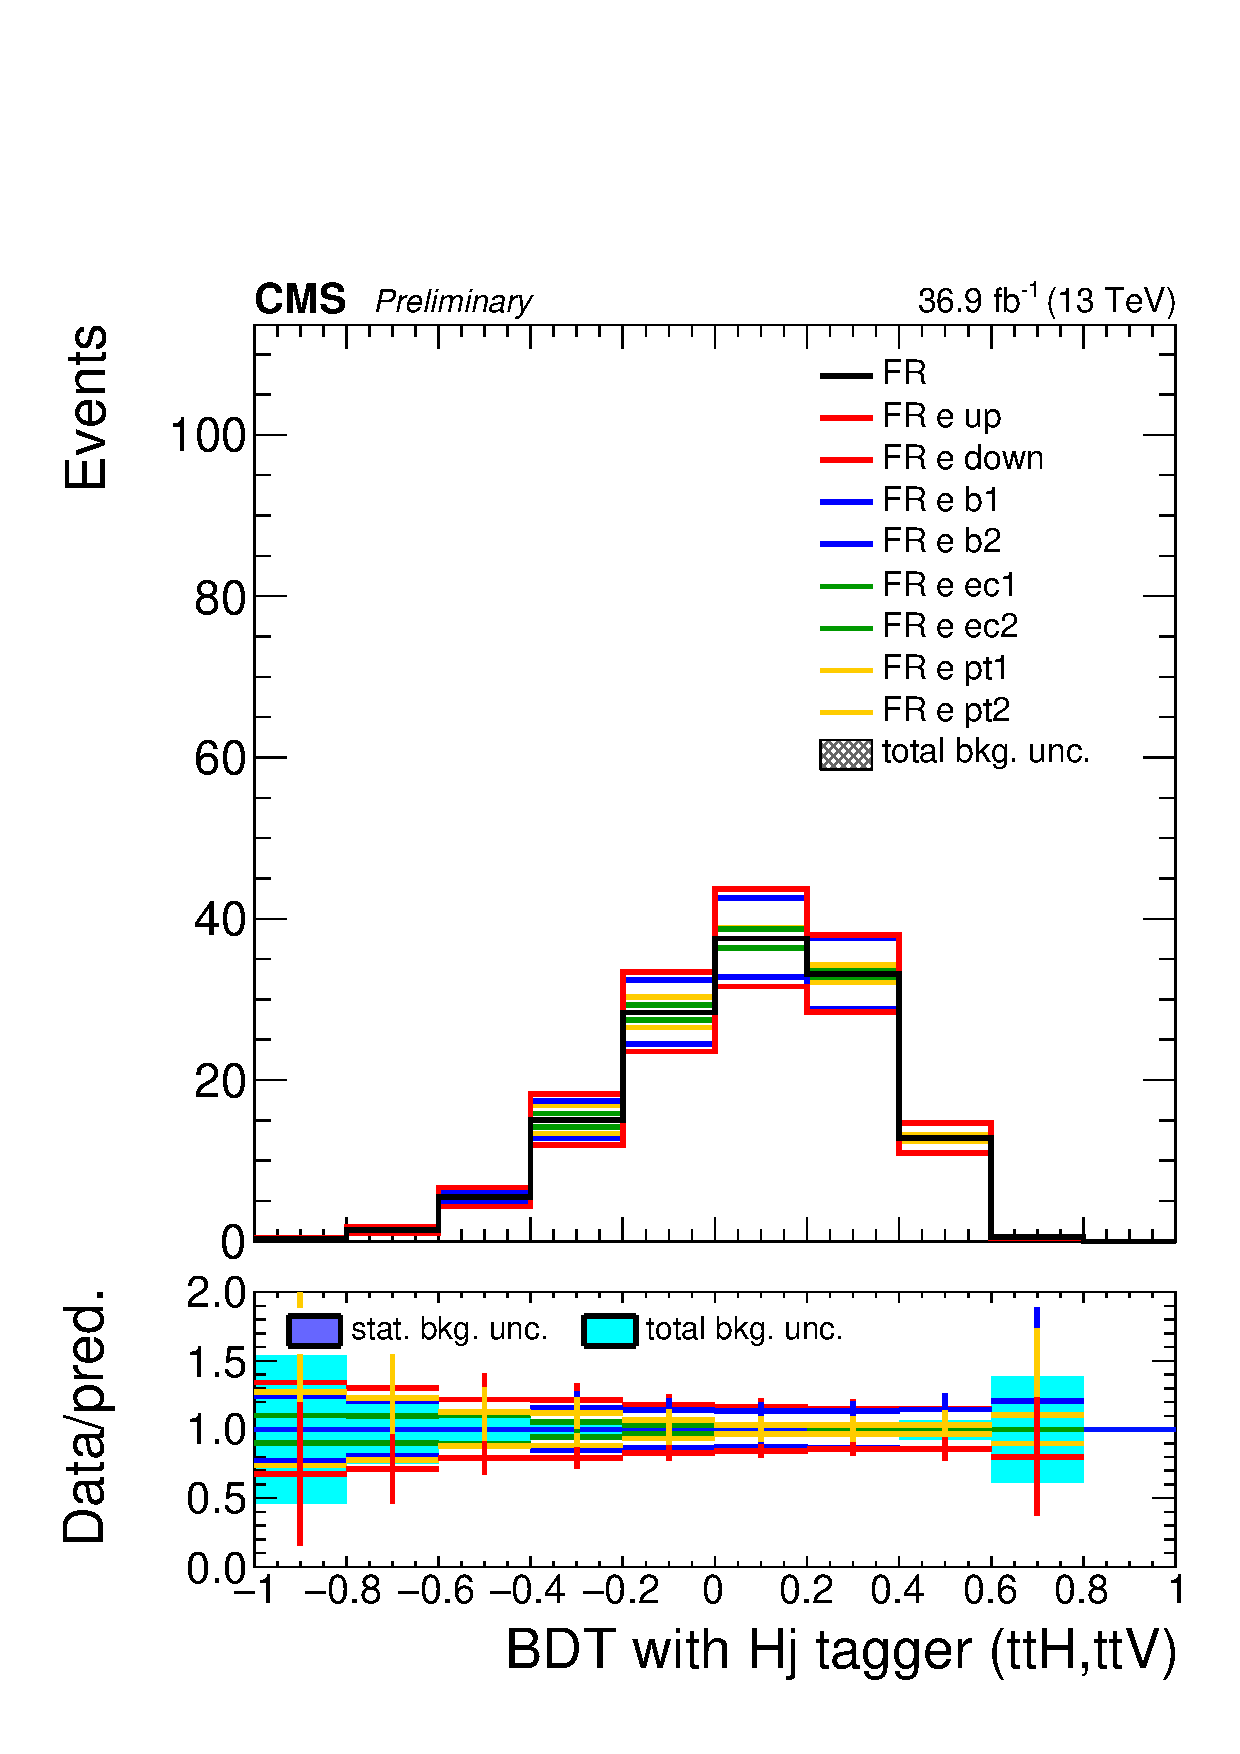
\includegraphics[width=0.32\textwidth]{ch10_figs/kinMVA_2lss_e_ttV_withHj.pdf}
        \caption[Variations in discriminant shape due to fake rate systematics]{Shape variations on the fake lepton background from shifts and distortions
          of the measured data fake rate bins within uncertainties ($\pm$1$\sigma$). 
          The shapes resulting from varying the fake rate up and down are in red. Barrel, endcap region shifts are in blue, green respectively. Variations as a function
          of lepton \pt are in yellow. The top (bottom) row is for variations to the muon (electron) fake rates respectively. The total background uncertainty in the
          data/prediction ratio is purely statistical uncertainty from each bin.}
        \label{fig:FRvars_shape}
\end{figure}

For the background due to charge mis-assignments, the estimation method is validated in two separate control regions.
The first control region is enriched in DY events, and is the same region used for measuring the charge flip rates.
The second control region is enriched in \ttbar events, and is defined by requiring a same-sign tight electron pair with invariant
mass within 30 GeV of the Z mass (to ensure charge flip events), the same b-jet requirement as the signal region,
and exactly 2 or 3 preselected jets. The widened mass window around the Z and the jet requirements ensure \ttbar events in this
control region. The purpose for the \ttbar-enriched control region is to verify the extent to which the good data/MC agreement observed
in the DY-enriched control region, deteriorates in the presence of multiple hadronic jets - which are present in the signal region. 
The data/MC agreement in this region therefore drives uncertainty estimation on the charge flip background. 
The data/MC agreement in the DY enriched, and in the \ttbar enriched control regions
for relevant variables is shown in Figure~\ref{fig:chargeFlip_cr} in the top and bottom rows respectively.
Based on the data/MC agreement in the control regions, and the statistical uncertainty of measured probabilities,
a 30$\%$ rate uncertainty is assigned to the charge flip background.


\begin{figure}[htb]
        \centering 
        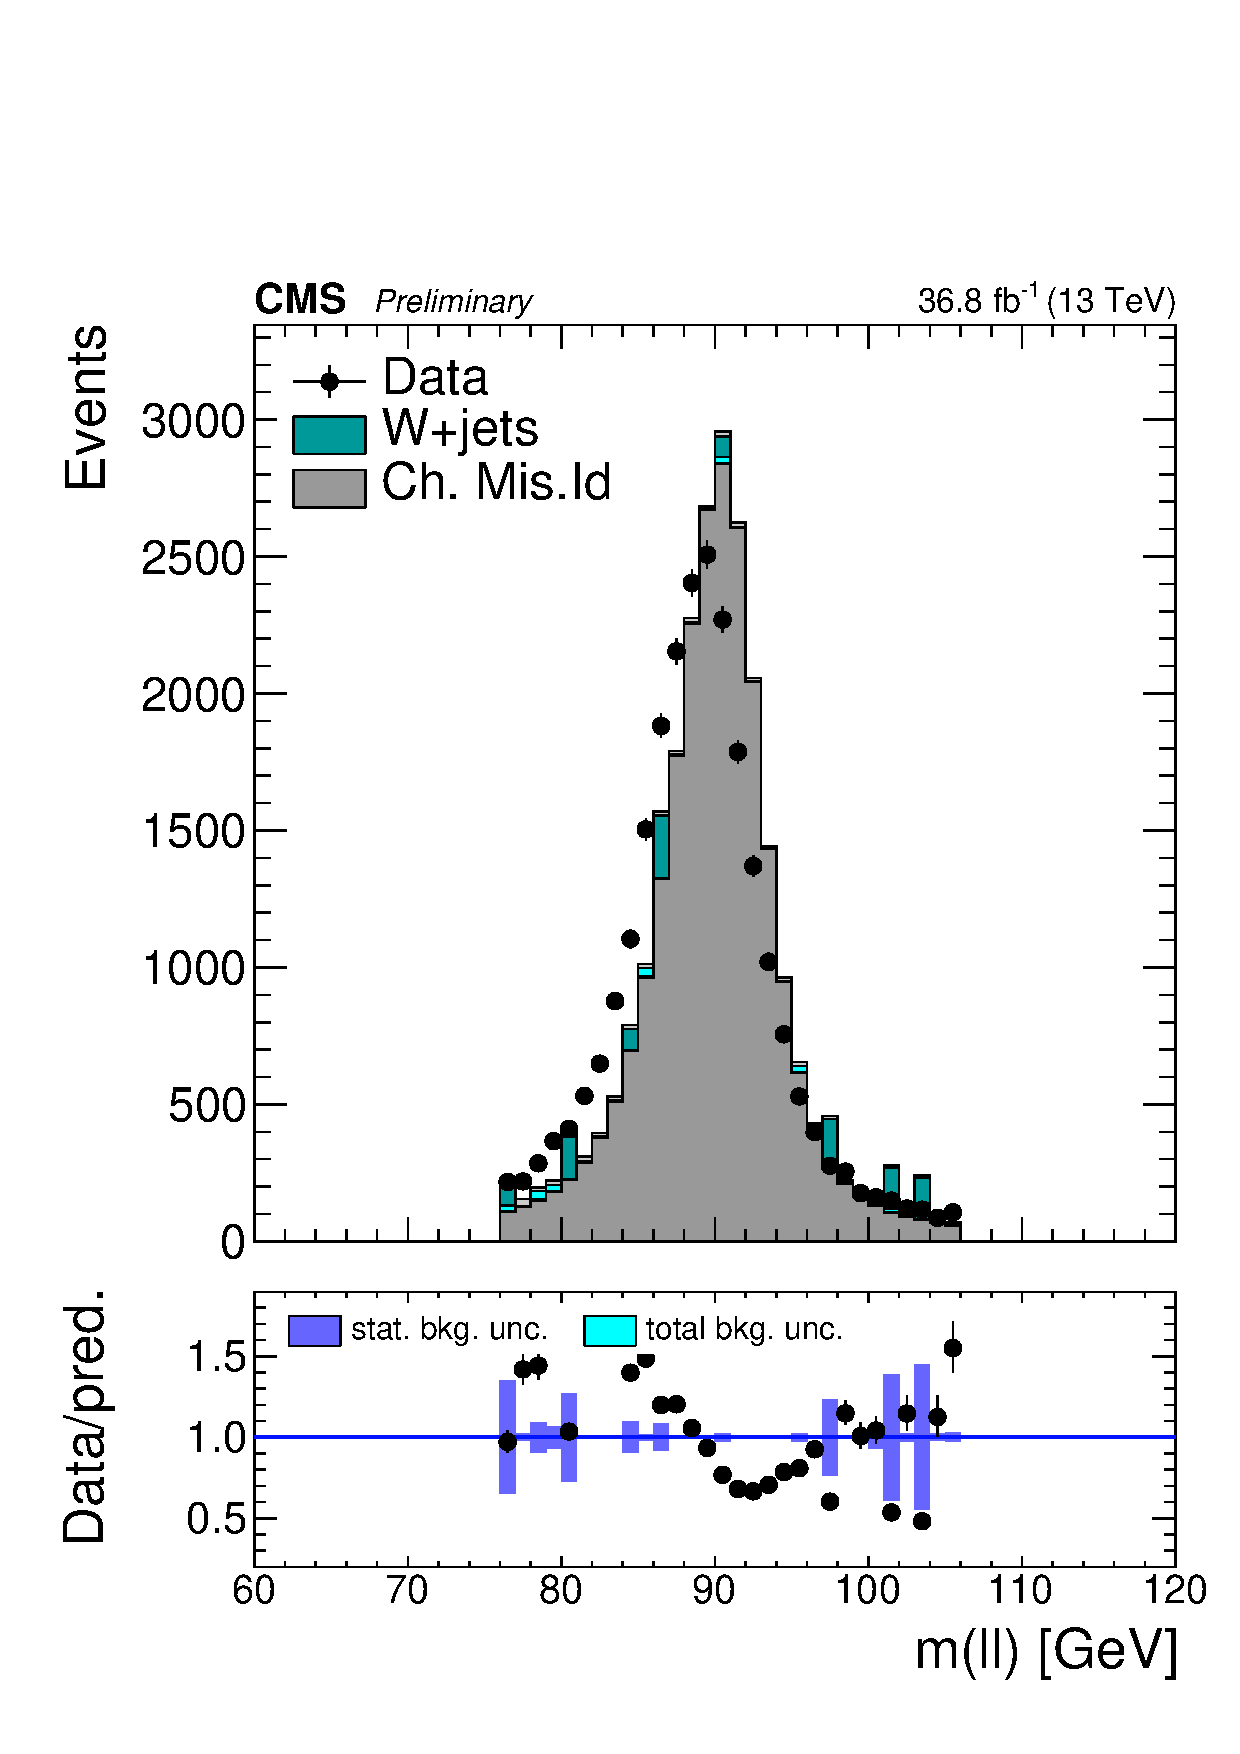
\includegraphics[width=0.32\textwidth]{ch10_figs/chargeFlip_closureDy/minMllAFAS.pdf}
        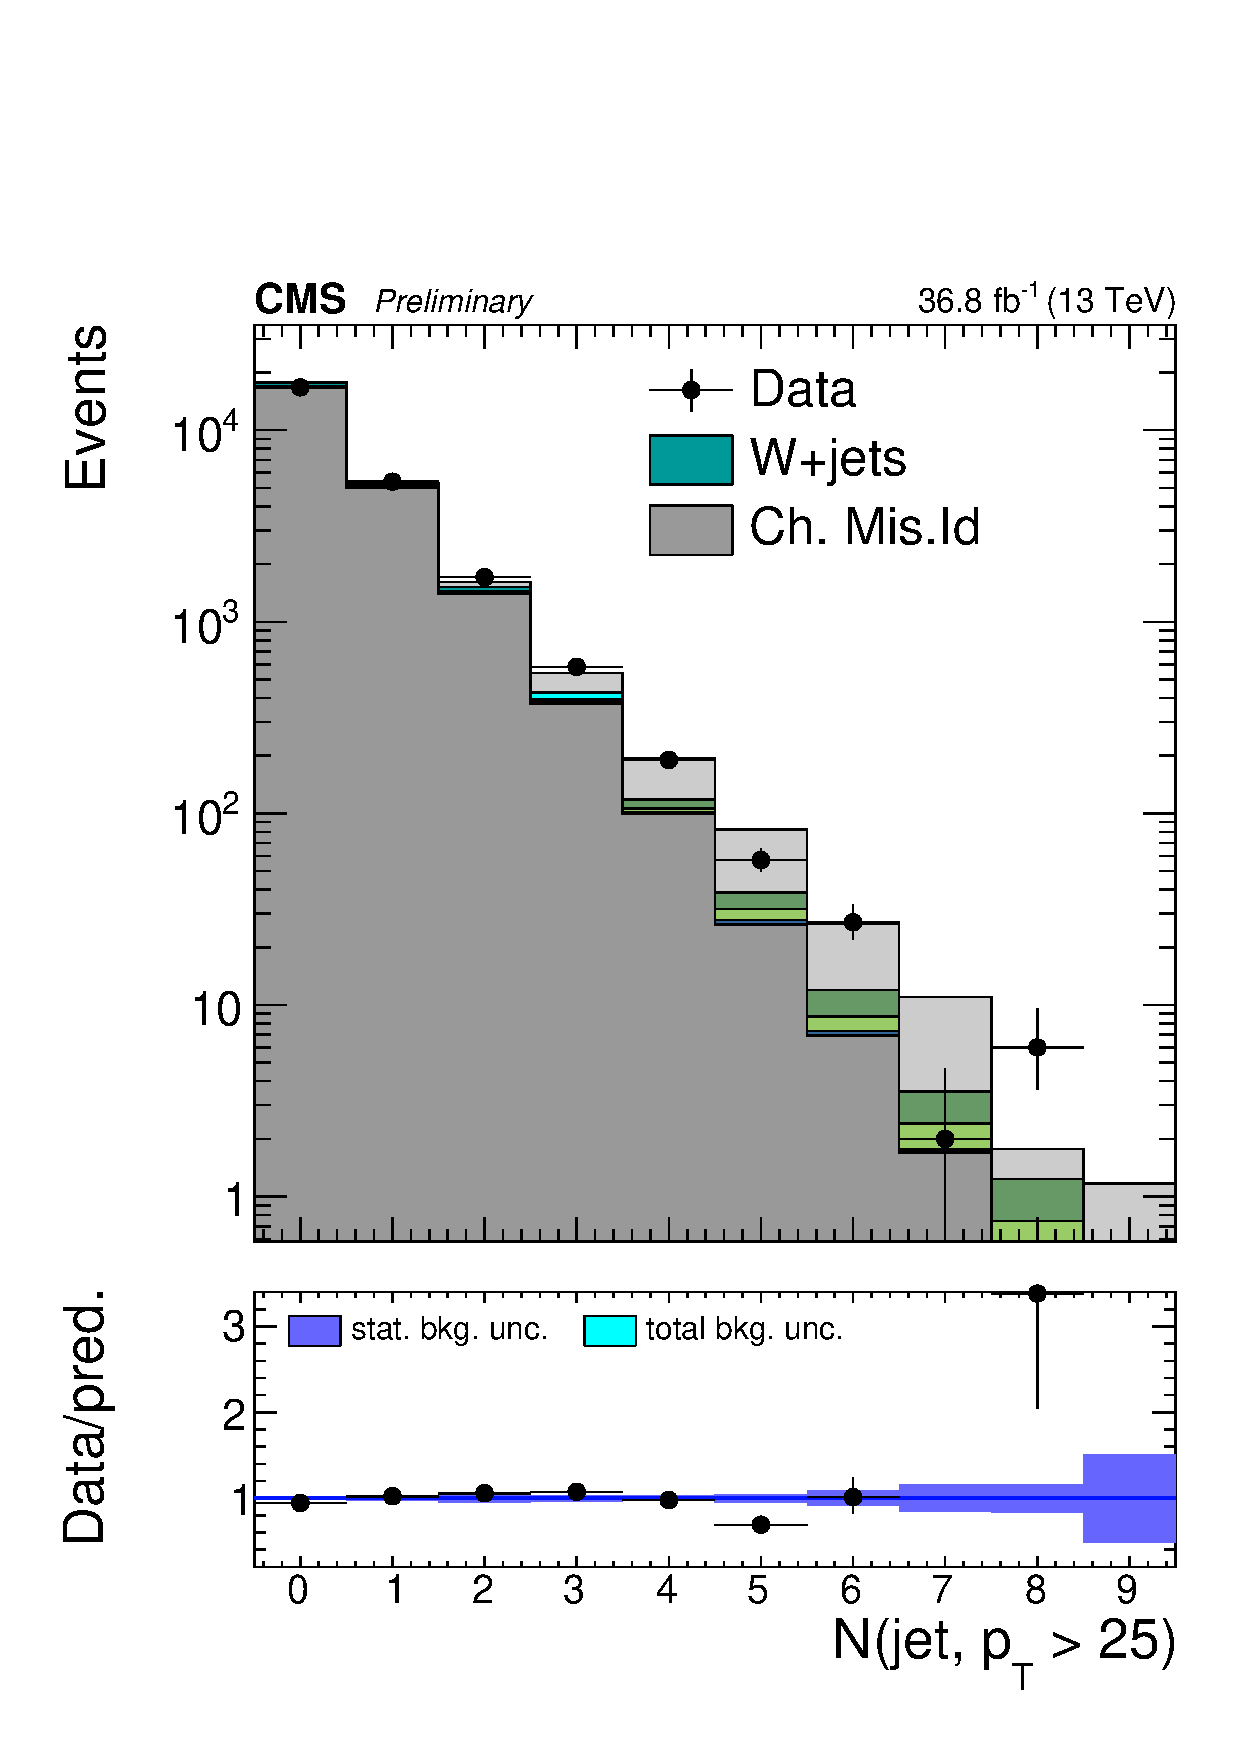
\includegraphics[width=0.32\textwidth]{ch10_figs/chargeFlip_closureDy/nJet25.pdf}
        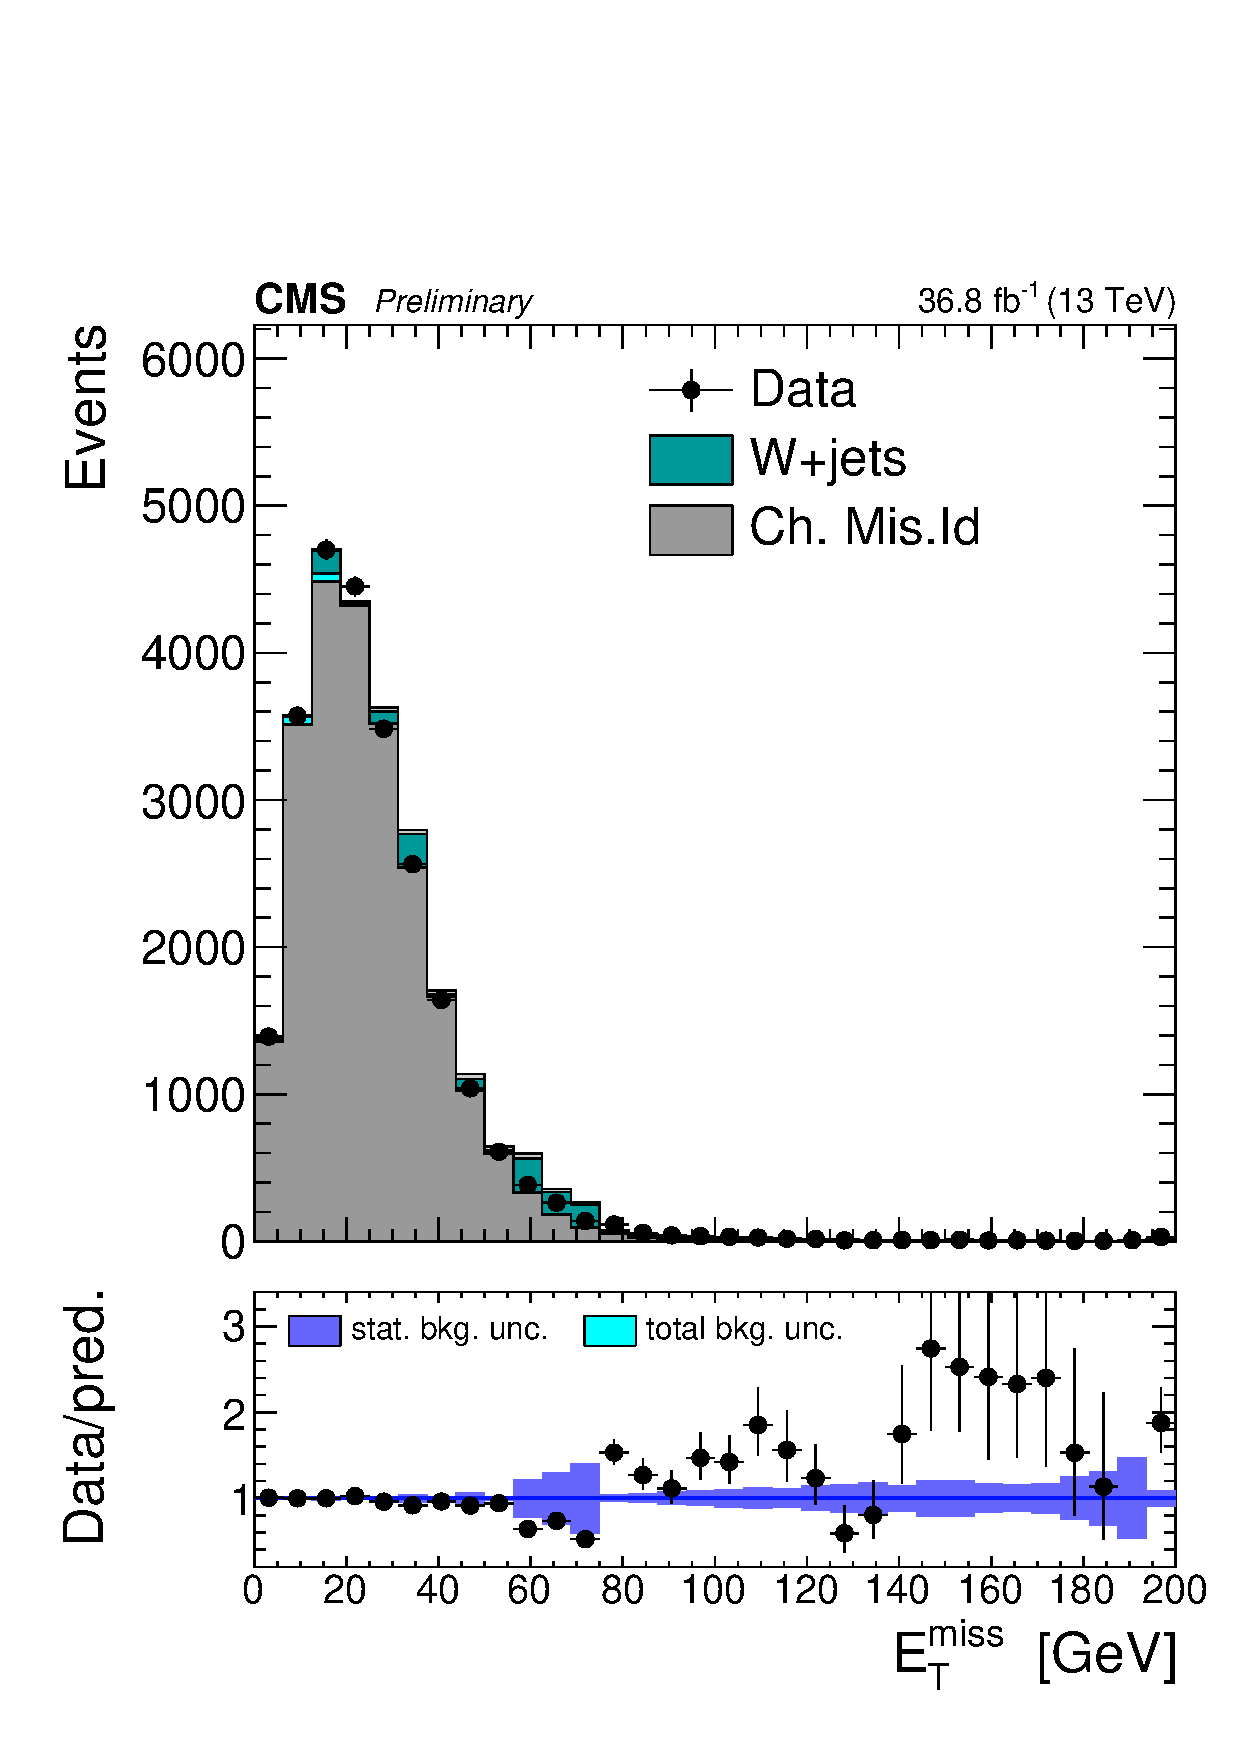
\includegraphics[width=0.32\textwidth]{ch10_figs/chargeFlip_closureDy/met.pdf}\\
        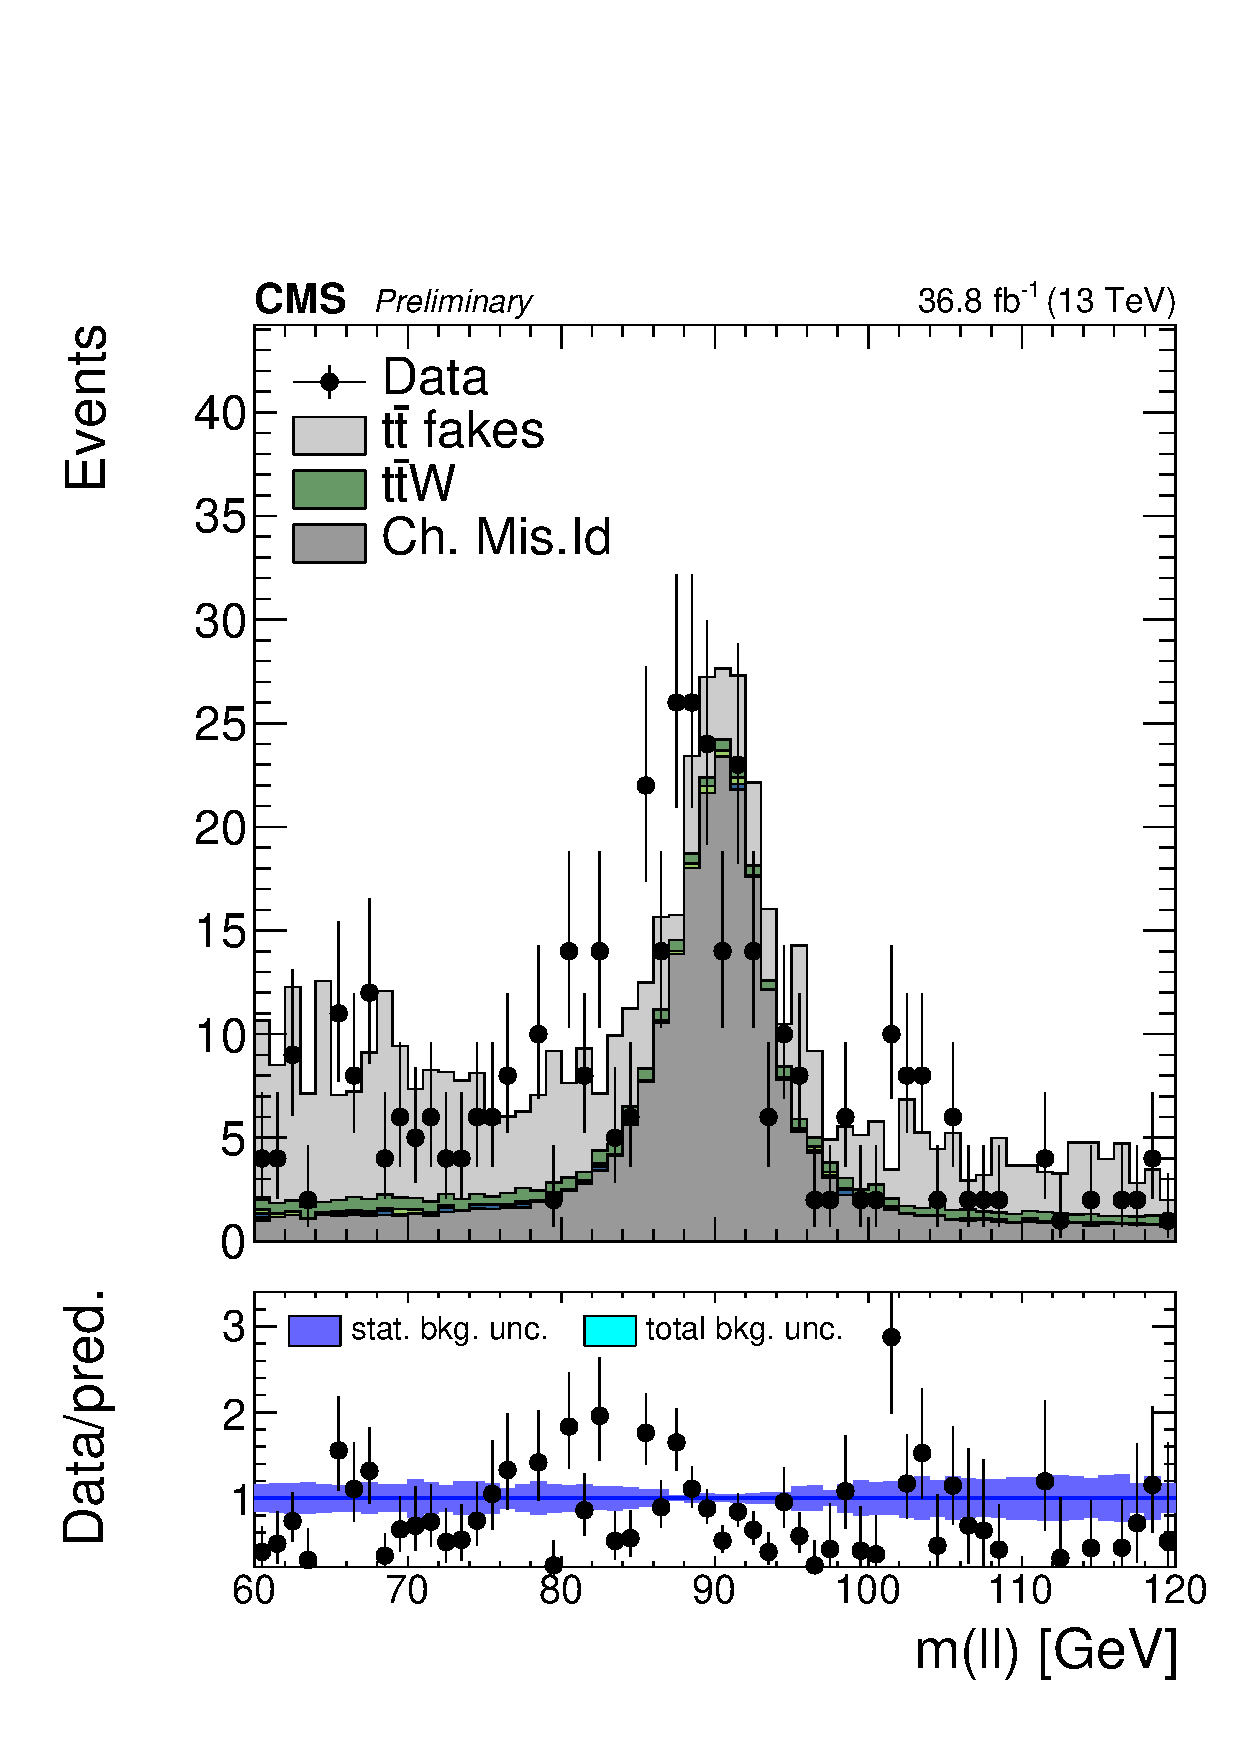
\includegraphics[width=0.32\textwidth]{ch10_figs/chargeFlip_closureTt/minMllAFAS.pdf}
        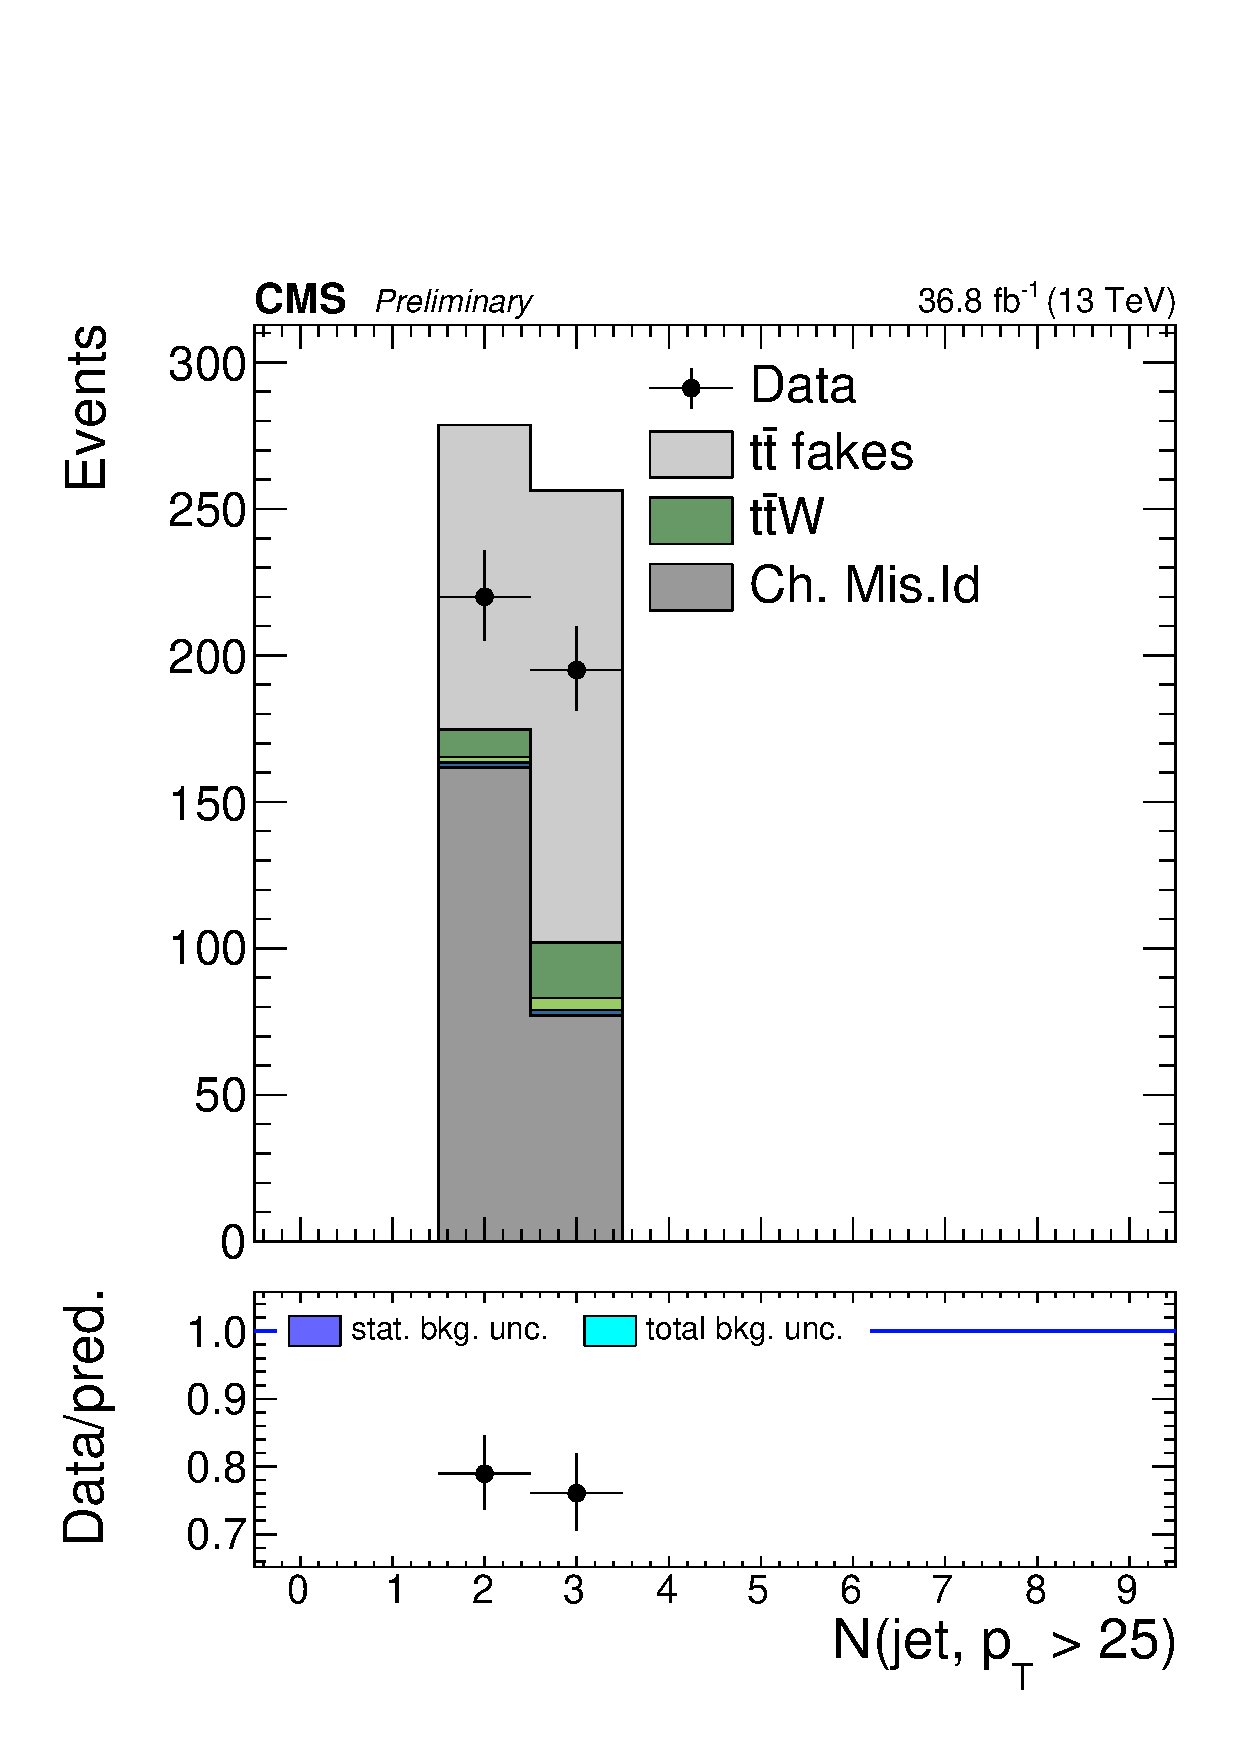
\includegraphics[width=0.32\textwidth]{ch10_figs/chargeFlip_closureTt/nJet25.pdf}
        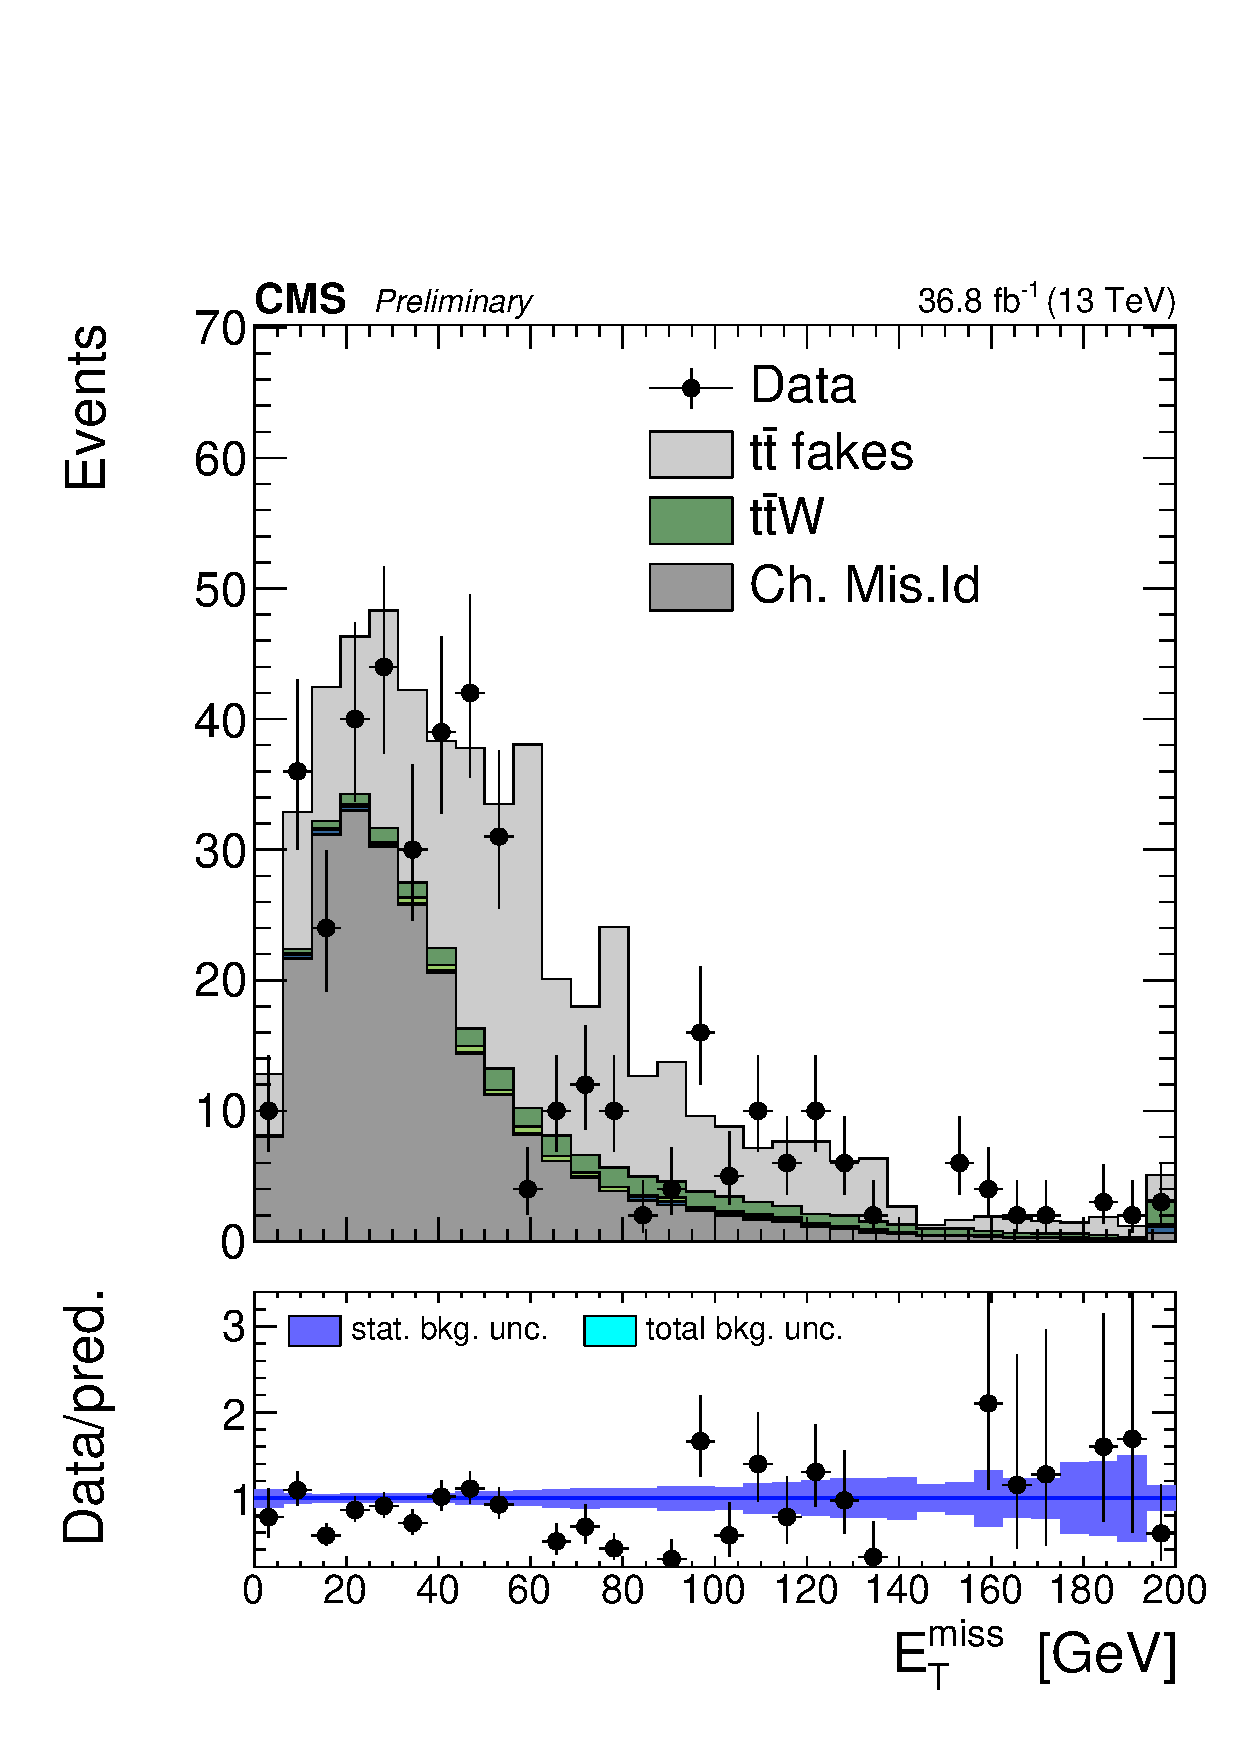
\includegraphics[width=0.32\textwidth]{ch10_figs/chargeFlip_closureTt/met.pdf}
        \caption[Data/MC agreement in charge flip control regions]{Data/MC agreement in Dilepton invariant mass (left), jet multiplicity (middle), and \met (right) variables
        in the DY enriched control region (top row) and \ttbar-enriched control region (bottom).}
        \label{fig:chargeFlip_cr}
\end{figure}
